%% wlkr
\documentclass{article}
\usepackage[hidelinks]{hyperref}
\usepackage{graphicx}
\usepackage{float}
\usepackage{listings}
\usepackage{tikz}
\usepackage{pdfpages}
\usetikzlibrary{positioning}
\usepackage[margin=1in]{geometry}

\lstset{
  basicstyle=\scriptsize, %or \small or \footnotesize etc. 
  commentstyle=\color{red},
  keywordstyle=\color{blue},
  showstringspaces=false,
  breaklines=true,
  aboveskip=1em,
  belowskip=1em
}

\begin{document}
\title{Bird Density, with Edge ML}
\author{Ryan Walker, Jin Seo}

% make the title area
\maketitle

\tikzset{%
  every neuron/.style={
    circle,
    draw,
    minimum size=1cm
  },
  neuron missing/.style={
    draw=none, 
    scale=4,
    text height=0.333cm,
    execute at begin node=\color{black}$\vdots$
  },
}

\section{Introduction}
Biologists have been aiming to understand bird migration for decades. Various custom hardware has been developed for doing this \cite{BirdTracking}, however is it costly an requires capture and release of the bird. We are proposing the design, construction and deployment of a device that resides in a stationary location. This device is equip with a microphone and microcontroller, and by using machine learning techniques \cite{ML1} \cite{ML2} can detect and speciate various types of birds. In addition the device will also be able to record various types of environmental data for cross-correlation with bird density in post processing. Following the successful deployment we desire to make a bird density heat map of various regions and to undestand how it changes over time.

\section{Machine Learning on the Edge}
\begin{center}
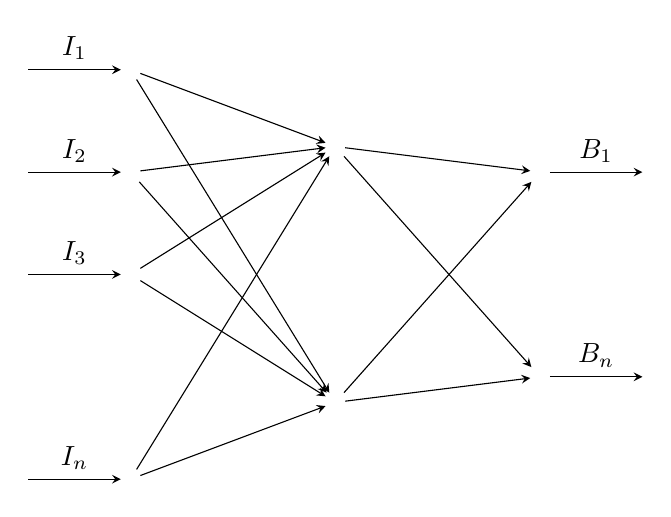
\begin{tikzpicture}[x=1.3cm, y=1.3cm, >=stealth]
\foreach \m/\l [count=\y] in {1,2,3,missing,4}
  \node [every neuron/.try, neuron \m/.try] (input-\m) at (0,2.5-\y) {};

\foreach \m [count=\y] in {1,missing,2}
  \node [every neuron/.try, neuron \m/.try ] (hidden-\m) at (2,2-\y*1.25) {};

\foreach \m [count=\y] in {1,missing,2}
  \node [every neuron/.try, neuron \m/.try ] (output-\m) at (4,1.5-\y) {};

\foreach \l [count=\i] in {1,2,3,n}
  \draw [<-] (input-\i) -- ++(-1,0)
    node [above, midway] {$I_\l$};

\foreach \l [count=\i] in {1,n}
  \draw [->] (output-\i) -- ++(1,0)
    node [above, midway] {$B_\l$};

\foreach \i in {1,...,4}
  \foreach \j in {1,...,2}
    \draw [->] (input-\i) -- (hidden-\j);

\foreach \i in {1,...,2}
  \foreach \j in {1,...,2}
    \draw [->] (hidden-\i) -- (output-\j);

\end{tikzpicture}
\end{center}

Machine learning and AI have been popular topics in the last couple of years, especially the use of neural networks in classification algorithms. A neural network is a collection of artificial neurons which can loosely model the neurons in a biological brain. They are connected is a way that allows data to propagate through them, each neuron connection (edge) has a weight associated with it, this weight either increases or decreases the strength of the signal at a connection. The neurons are arranged in ``layers", the first and last layers are known as the input and output layers respectively, and the middle layers are known at the hidden layers. ``Training" a neural network is the automated process of adjusting the weights on a sample dataset so that the output gives the requred value for a given input. As an example, if were given a problem to classify 1000 pictures into either ``hotdog" or ``not hotdog", where the images were 250 pixels by 250 pixels. You would start by:

\begin{itemize}
\item Manually label a sufficiently large section of the dataset (say 500 pictures)
\item Introduce 62500 input neurons ($250 \cdot 250$)  
\item Introduce 1 output neurons (Hotdog or not hotdog)  
\item Train the network so output says hotdog for all the hotdog pictures, and not hotdog for all the not hotdog pictures
\item When you then feed in puctures it hasn't seen before, it should classify the remaining data correctly
\end{itemize}

The accuracy is given by the ratio of correct classifications to incorrect classifications. It has not been until recently that these applications have moved into edge compute, meaning all the processing is run on the device as apposed to cloud. We propose to design a NN (Neural Network) that can be run on a STM32 microcontroller for classification of various birds. As this is such a rapidly expanding field there are various software implementations developed for embeded applications \cite{CMSIS} \cite{TF}. 

\section{Signal processing}
This project is required to utilize several signal processing techniques. Some of these techniques could be included filters, discrete Fourier transforms, and so on. Filters are necessary to improve the quality of the bird calls and remove unwanted noises. In addition, in order to come up with digitized data from acoustic analog signals, other techniques could be applied such as Discrete wavelet transform or mel-frequency cepstrum. In this case, MATLAB can be used for simulation.

\subsection{Mel Spaced Filter Bank}
Human hearing sensitivity works in a very nonlinear way. For a human, there is a stark difference between a signal that is 50hz and a signal that is 150hz. However is it almost impossible to notice a difference between a a 10khz signal and a 11khz signal. The mel scale has been developed to represent this. It it shown in Equation \ref{mel-eq} and is plotted in Figure \ref{mel}. 

\begin{equation}
M(f) = 1125 \cdot log(1+\frac{f}{700})
\label{mel-eq}
\end{equation}

\begin{figure}[h]
\centering
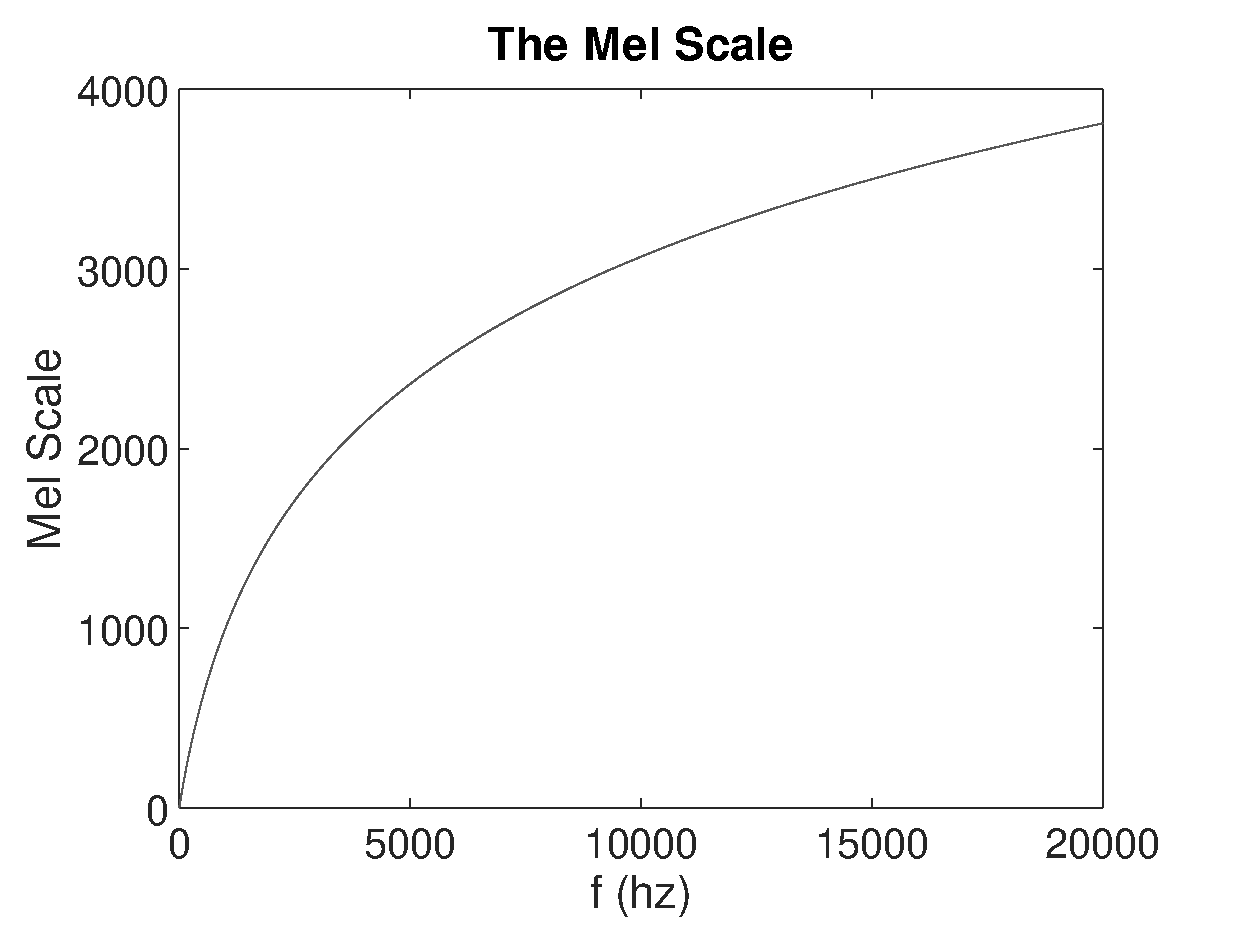
\includegraphics[width=9cm]{mel.eps}
\caption{The Mel Scale}
\label{mel}
\end{figure}

To get more adequate feature extraction we are going to use a mel spaced filter bank. This effectively maximizes the features extracted as a function of the mel scale. The filter array is shown in Figure \ref{FA}. In this example we have implemented ten filters for visulizing purposes, however in practice we are going to implement over twenty.

\begin{figure}[H]
\centering
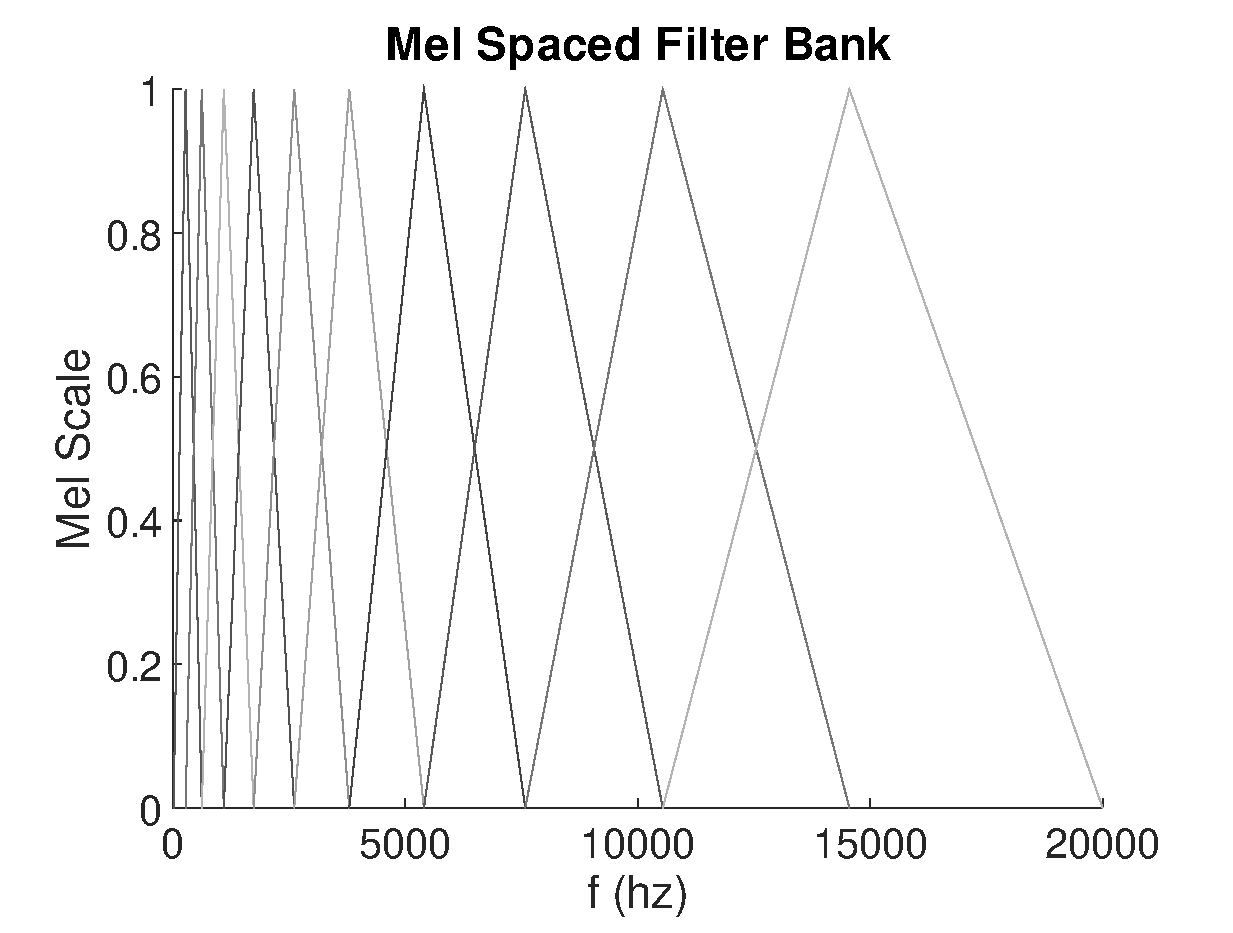
\includegraphics[width=9cm]{FA.eps}
\caption{The Mel Scale}
\label{FA}
\end{figure}

\section{Software} In the project we are planning on using Matlab/Simulink for any filter design, C/C++ for embedded code and possibly some python for post processing.

\section{Hardware}
The hardware will need to be battery powered in order to collect data over extended periods of time. We are currently targeting the specifications below.

\begin{center}
\begin{tabular}{ c | c }
Spec             & Metric\\ 
\hline 
Battery Life     & 1 week\\
Compatable Birds & 10    \\
Cost (QTD 100)   & $<\$30$  \\
\end{tabular}
\end{center}

It should be inexpensive so it becomes feasible to deploy many devices and should be completely stand alone. In addition it should have a wiresless uplink/downlink to transmit data to and from a computer.

\subsection{Microcontroller}
In addition to having experience with the STM32 family of microcontrollers, TensorFlow Embedded \cite{TF} has extensive documentation for implementation on the STM32F746 \cite{STM}. This part has 1MB flash, 320k RAM and runs at 216Mhz. TensorFlow embedded is designed to run on 20k of flash, so we will have more than enough space for the NN and application code.

\subsection{Microphone}
The device will contain a microphone that will be used to record ambient noises. A suitable microphone has not yet been selected.

\subsection{Architecture}
\begin{itemize}
\item{\textbf{MCU:} STM32F746.}
\item{\textbf{SD card:} For recording data.}
\item{\textbf{18650 Cell:} 2x 18654 Li-ion cells for power.}
\item{\textbf{Microphone:} Microphone for recording sound.}
\item{\textbf{Temperature Sensor:} Temperature sensor for recording ambient temperature.}
\end{itemize}

\section{Data Harvesting and Conditioning}
In order to train the neural net, we require a great deal of data. This was gatherd from a website where bird listeners post sounds of birds \cite{Bird}. To this day we have gathered and labeled 589 crow samples, of which roughly half are not crows and 691 sanpiper samples to which roughly half are not sanpipers. We did this using the workflow outlined below.

\subsection{Harvesting}
The script below harvest the data from a given bird.
\lstinputlisting[language=bash]{../NN/data/fetch.sh}

\subsection{Labeling}
The labeling process was done manually, it was done with the script below essentually this script will hunt through a file and find sound files, then it will chunk off a 1s piece and play it, if the user presses 'y' then it will save the file down as ``n\_crow" if the user pressed 'n' then it will save the file down a ``n\_Notcrow", where n is an incremented integer.
\lstinputlisting[language=python]{../NN/data/splice.py}

\subsection{Conditioning}
Our neural network is deigned to accepts frequency data, not sound data. So there is some conditioning required beforehand. This script opens up the output files from the last script and preforms a FFT. It then reduces the number of bins to something more manageable, right now we are using 128 input neurons, so there are 128 fft bins. It then saves all this to a single json file. 
\lstinputlisting[language=python]{../NN/data/fft.py}

\section{The Neural Network}
We chose Tensorflow for out neural network design because one you train up a model, you have the ability to convert it to a ``tflite" model which can be run on a microcontroller using tensorflow lite. We then built the model structure and trained the model. Our current model is shown in Figure \ref{model}, it has 128 input neurons on the input layer (for our 128 fft bins) 128 neurons on the one hidden layer and 1 neuron on the out (either crow or not crow). The script starts by randomly splitting our dataset into the training and validation set, where the training set it used for the training while the validation set is used for validation after the training is complete, that is to say the network has no knowledge of the validation set when adjusting the weights. After this process our network got \textbf{93\% accuracy on the validation set}
\lstinputlisting[language=python]{../NN/audio/src/main.py}

\begin{figure}[H]
\centering
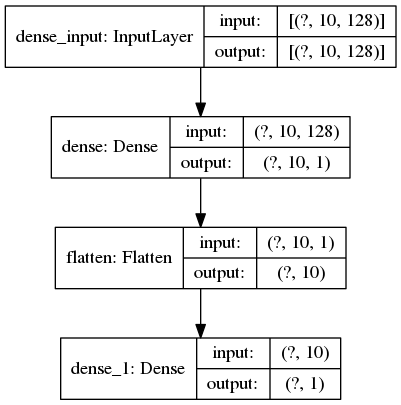
\includegraphics[scale=0.3]{../NN/audio/src/model.png}
\caption{Current Model}
\label{model}
\end{figure}
\newpage

\section{Hardware}
The first revision of the hardware is finished and we have connected to the microcontroller. The physical hardware is shown in Figure \ref{hardware} while the schematic is shown in Figure \ref{sch1} and \ref{sch2}. We got a PCB manufactued overseas ans placed all the SMD components onto it.
 
\begin{figure}[H]
\centering
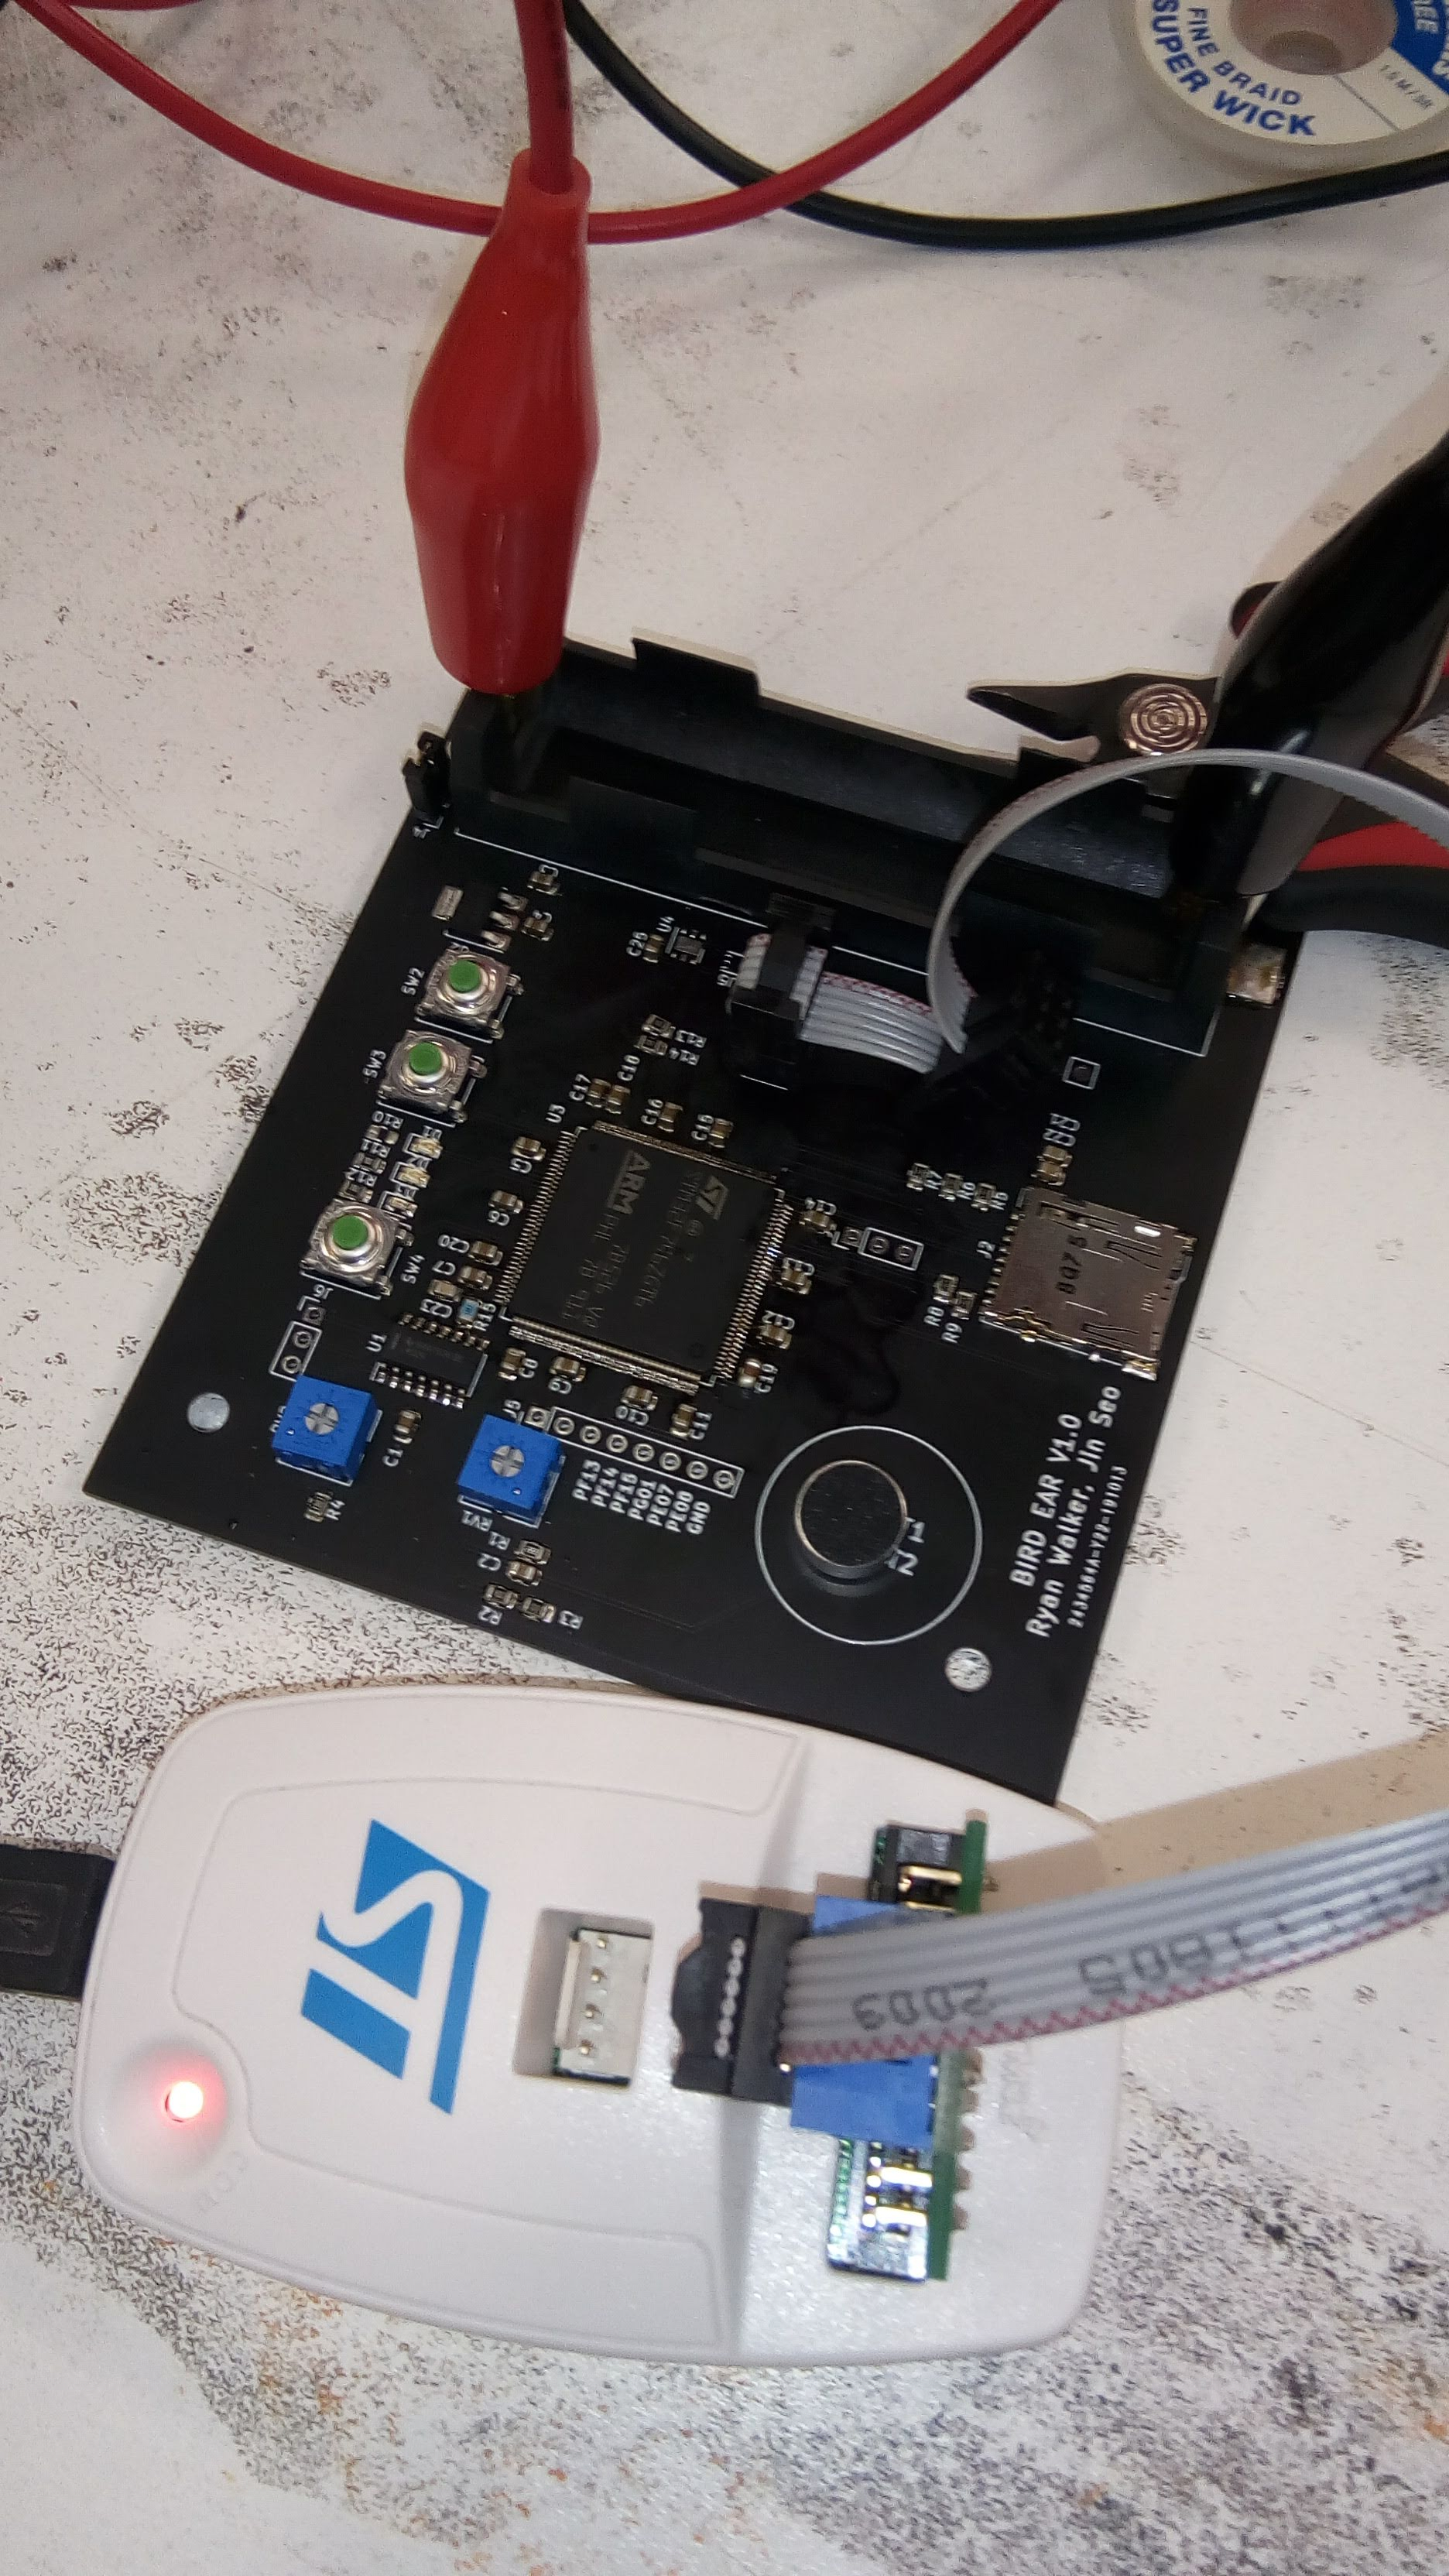
\includegraphics[scale=0.15]{../birdEar/img/be.jpg}
\caption{Hardware}
\label{hardware}
\end{figure}

\begin{figure}[H]
\centering
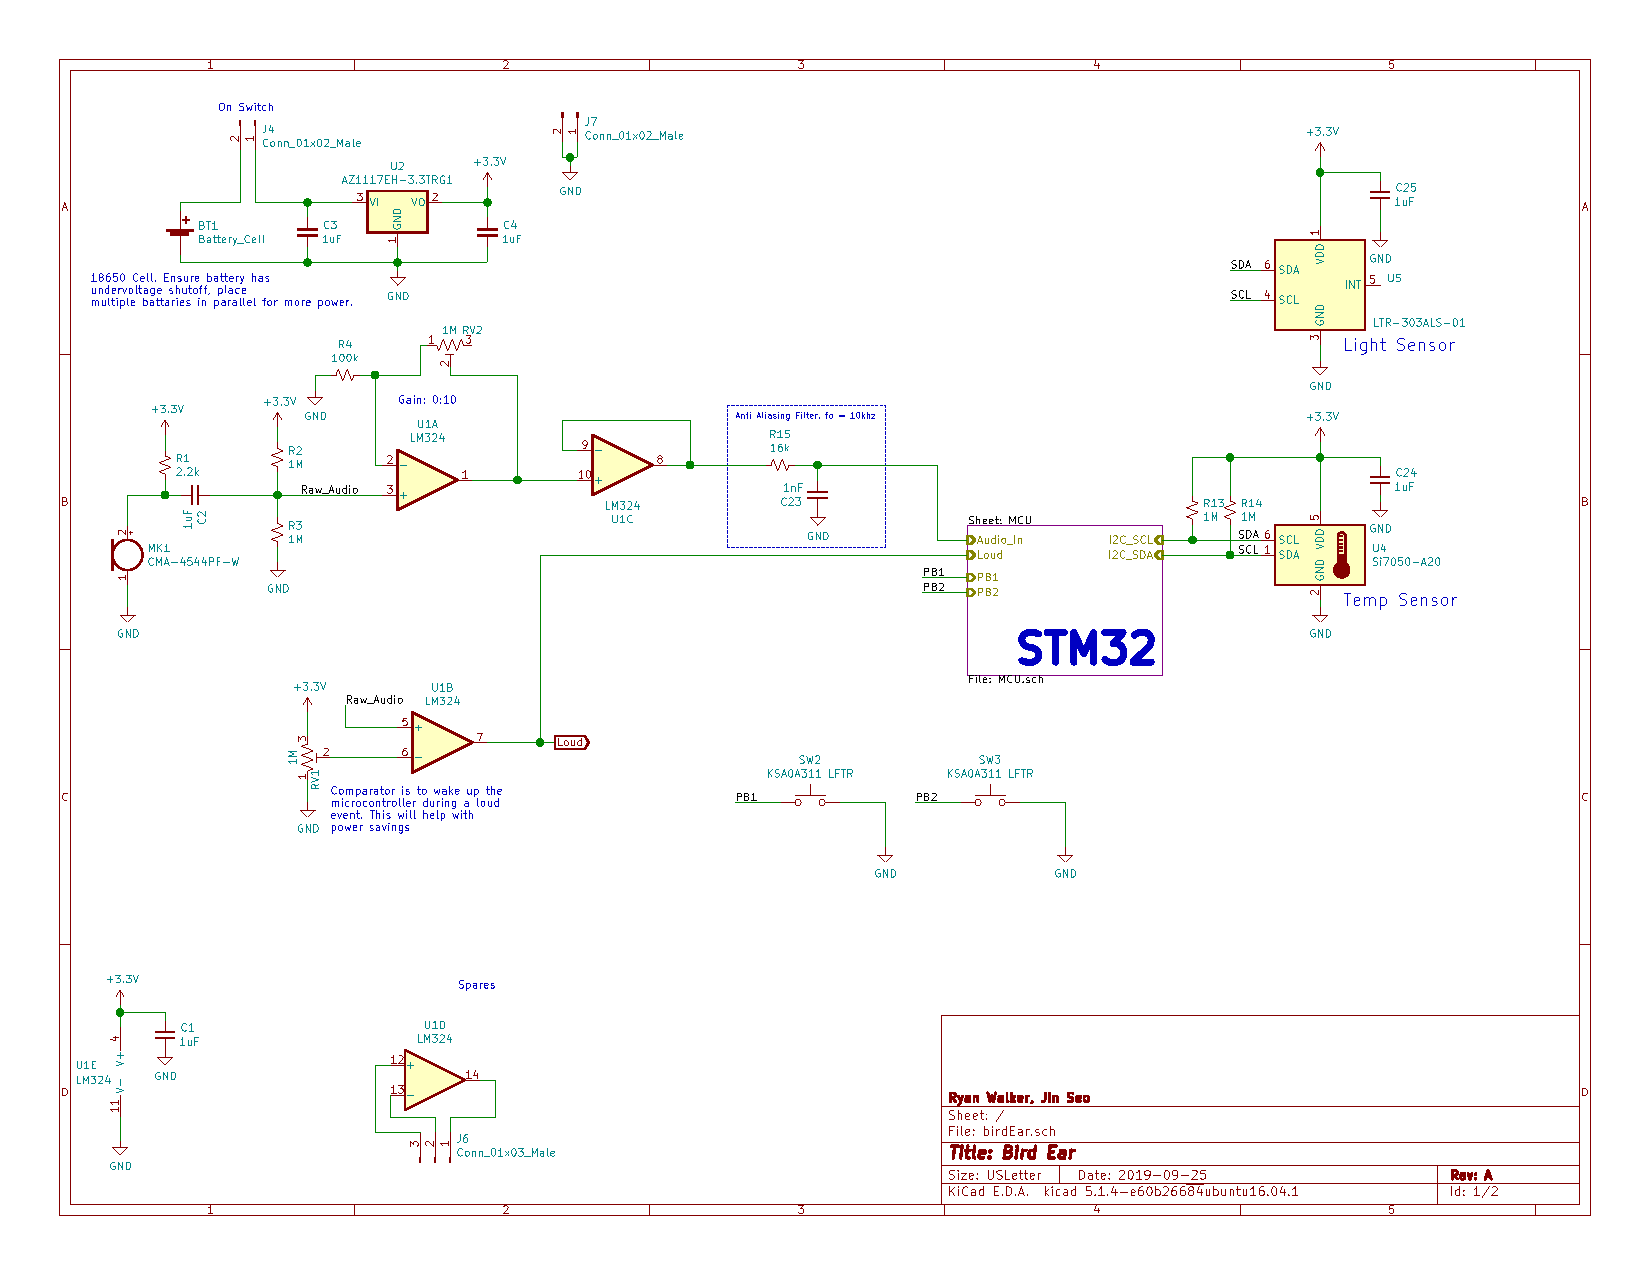
\includegraphics[scale=0.7, angle=90, page=1]{../birdEar/plot/birdEar.pdf}
\caption{Schematic - page 1}
\label{sch1}
\end{figure}

\begin{figure}[H]
\centering
\includegraphics[scale=0.7, angle=90, page=2]{../birdEar/plot/birdEar.pdf}
\caption{Schematic - page 2}
\label{sch2}
\end{figure}

\section{Next Steps}
The next steps of the project are...

\begin{itemize}
\item Implement mel-spaced frequency array.
\item Increase the number output neurons to 2, so we can classify between crows and sandpipers. 
\item Add another three types of birds to the dataset.
\item Research "VGG like feature extraction".
\item Implement microcontroller firmware for audio sampling.
\item Implement neural network on the microcontroller.
\item Deploy the device in the field.
\end{itemize}

\begin{thebibliography}{1}

\bibitem{BirdTracking}
Bird Tracking Hardware.
\url{https://atstrack.com/animal-class/avian.aspx} [Accessed June 22, 2019]

\bibitem{ML1}
Stowell, Wood, Pamuła, Stylianou4, Glotin "Automatic acoustic detection of birds through deep learning: the first Bird Audio Detection challenge"
\url{https://arxiv.org/pdf/1807.05812.pdf}

\bibitem{ML2}
Ilyas Potamitis, "Deep learning for detection of bird vocalisations"
\url{https://arxiv.org/pdf/1609.08408.pdf}

\bibitem{CMSIS}
CMSIS NN Software Library
https://www.keil.com/pack/doc/CMSIS/NN/html/index.html

\bibitem{TF}
TensorFlow Lite for Microcontrollers
https://www.tensorflow.org/lite/microcontrollers/overview

\bibitem{STM}
ARM® Cortex®-M7 STM32F7 Microcontroller IC 32-Bit 216MHz 1MB (1M x 8) FLASH 100-LQFP (14x14)
https://www.digikey.ca/product-detail/en/stmicroelectronics/STM32F746VGT6/497-15819-ND/5287178

\bibitem{Bird}
xeno-canto is a website dedicated to sharing bird sounds from all over the world.
https://www.xeno-canto.org/

\bibitem{BirdCallIdentifier}
Bird Call Identifier.
\url{https://web.wpi.edu/Pubs/E-project/Available/E-project-042910-001603/unrestricted/Bird_Call_Identification_MQP_2010.pdf} [Accessed April 29, 2010]

\end{thebibliography}

\end{document}
